\chapter{Evaluation}
Evaluation of the performance of a system is one of the most important part of the process in implementing a new system. For the Twitter spelling error correction system evaluation was particularly important to justify building an entire system instead of using existing software systems. In this chapter, the dataset used for experimentation is described, an evaluation metric used to compare the effectiveness of the new systems created, and the results of the various investigations into the questions posed in section 1 are performed and analysed.

\section{The Data Set}
For a machine learning task, such as the Twitter spelling error correction system designed and implemented throughout this report, the key to the accuracy and effectiveness of the system is the amount and quality of the data. Machine learning systems, by definition, learn from the data that is supplied to them and therefore need many examples to work from to further their knowledge and provide the most accurate results. For this task there were two forms of data required to train and evaluate the system.

Firstly, training data was required in order to build a system that could know what a spelling error looked like and could subsequently correct that error to the word that the user originally intended to type or should have typed. For this task, the length of the texts was particularly important in order to provide enough variety to model as much of the commonly used English language as possible in order to decrease the number of false positive spelling errors detected. As well as length, the spelling in the texts must be of a high quality to ensure that any corrections suggested by the system are more likely to be correct than if the training data is filled with errors. 

Taking the preceding requirements and the availability of corpora within the University into account the Associated Press Worldstream (APW) \cite{} was chosen as one of the main training texts for the system along with the New York Times (NYT). These corpora encompass news stories as circulated by the Associated Press (AP) and New York Times newswires respectively. AP estimates that around 200 new stories are published each day \cite{} and therefore obviously there was a lot of text data that could be used to train the system. In addition to the amount of text, the quality of the texts was guaranteed to be of higher quality than some other text sources such as simply gathering text from websites online. As the news stories are published in newspapers and online they require high quality writing and are thoroughly edited before publication so represented a good example of well formed and spelled text. The final reason for choosing the APW was the recency of the publication. There are many corpora available for use but since Twitter is a fairly new and modern technology, the language that is used in the Tweets is reflected in this. Therefore, as the spelling error correction system was trying to model the language used by Twitter users it made sense to choose a set of text that was written more recently as it better modelled the modern English language.

As the APW corpus is large, a smaller subset of the corpus was selected for use in the system. The 2002 section of the corpus was selected as it represented a good amount of recent text (roughly 300MB) while not sacrificing the speed of training. Below is an example of the format of content in the APW corpus:

\begin{verbatim}
<P>
``We have a very short timetable to sit with Russia as 19 plus
1,'' Robertson said, explaining that NATO hopes to have the
structure of the new council ironed out by mid-May, when allied
foreign ministers meet in Reykjavik, Iceland, and approved at a
summit in Prague in November.
</P>
\end{verbatim}

By using this dataset with the system, the resulting dictionary contains just below 44000 unique words. This is a fairly good size of dictionary as the Oxford English Dictionary states that 50000 words represent over 95\% of the entire English language \cite{}.

To test the correction abilities of the spelling error correction systems there are two sets of data. The first set of data is part of the Birbeck Spelling Error Corpus \cite{} and is compiled from many misspellings of words taken from the students' of Sheffield University's Information Studies Department \cite{}. This dataset also pairs the spelling error with their respective correction which makes it easy to gauge the accuracy of a spelling error correction system on isolated-word errors.

Evaluating the accuracy on Tweets requires a large number of Tweets to correct. The Informatics department at The University of Edinburgh has collected and made available over 1TB worth of compressed Tweets\cite{}. This data was collected between DATEX and DATEY using a Hadoop cluster \cite{} that processes and stores over 1 million Tweets per day. The Tweets in this collection have been anonymised but still contain all of the other features of Tweets such as \emph{@Usernames} and \emph{#Hashtags}. An example of a Tweet from this dataset is presented below:

\begin{quote}
20091110083240 user1443 @user1444 What a great weekend for football, Cats beat KU and Cowboys beat the Eagles! web
\end{quote}

As well as recognising and correcting spelling errors in Tweets, it was important that the spelling error system recognised correctly spelled words and did not attempt to correct them. For this reason the data set included correctly spelled Tweets as well as Tweets containing spelling errors.

As was described in section 2 there were a great number of Tweets that are not in English as the Tweet collection process retrieves all Tweets that are visible publicly on Twitter. These foreign language Tweets can also contain Unicode characters that need to be handled without error.

Of course, as was alluded to in previous sections in this report there are many Tweets in the dataset with spelling errors. One example is:

\begin{quote}
20091110083322 user1801 jz came back home,almost had an accident jz now.... *haih* i hate freaking drivers who dont utilize thier signal lights!!!! argh!!!! =? web
\end{quote}

This Tweet, in particular, is a good example of the types of spelling errors that are common on Twitter. The user has used the contraction ``jz" to replace the longer word ``just" and the common spelling mistake of ``thier" when the correctly spelled word should be ``their". The format of all Tweets represents the date the Tweet was posted, the anonymised user name of the author, the Tweet message itself, and then the source application or website of the Tweet. Maintaining this structure was a vital part of the process to ensure that later systems, such as machine translation systems, which use the data can still use some of the data features other than the Tweets' text.

\section{Evaluation Metric}
\label{eval}
To evaluate how well the Tweet spelling error correction system worked an evaluation metric was devised to quantitatively measure the accuracy of each of the systems presented. The first step in this process was to gather sets of different Tweets to correct. To do this the 1TB Tweet file was randomly sampled until 100 Tweets were gathered for each set. By randomly sampling the data set the evaluation set was guaranteed to include spelling errors but also Tweets with no spelling errors which is an important test for the algorithms. 100 Tweets was selected in order to measure accurately a large number of Tweets while also keeping the human intervention in the system to a minimum. The process of randomly sampling the data was performed three times to create three sets of Tweet data. Using three sets of different Tweets increased the value of the evaluation metric by guaranteeing that none of the algorithms can be particularly suited to one set of data and that they must perform well over all sets to achieve a high rate of accuracy. The final amount of Tweet data that was selected to be used was three sets of 100 Tweets.

The next stage of the evaluation metric was to manually correct each of the evaluation sets of 100 Tweets and produce a new set of Tweets. If the Tweet was already spelled correctly the Tweet was copied to the new set verbatim. An example of this mapping from the set is:

\begin{quote}
20091110083322 user1801 jz came back home,almost had an accident jz now.... *haih* i hate freaking drivers who dont utilize thier signal lights!!!! argh!!!! =? web

20091110083322 user1801 just came back home,almost had an accident just now.... *haih* i hate freaking drivers who don't utilize their signal lights!!!! argh!!!! =? web
\end{quote}

To calculate the evaluation score for an algorithm using the above original to corrected Tweet mapping the system compares each system-corrected word, including the extra meta-data, to the human-corrected Tweet. From this comparison a percentage correctness could be calculated and this was the evaluation score for a particular algorithm on a particular Tweet. This process continued for all Tweets in one evaluation set until a single score was achieved by averaging over the percentage accuracy from each Tweet. Once the score for a single evaluation set is calculated, the process began again with the other two evaluation sets. The final score for the algorithm was then the average percentage correct over the three sets.

To further quantify the effectiveness of the various systems created time of execution was also calculated. The time of execution was only timed during the detection and correction phase and not the training phase as the times would largely be the same. The time was taken using Python's \emph{time.time()} \cite{} as is provided by the standard library. The time for execution was then simply the difference between the time taken at the end and the time taken at the beginning. The final output of the timing operation was then defined as the number of Tweets corrected per second.

\section{Accuracy of Generic Spelling Error Correction}
The first area of evaluation for the system was on generic spelling error correction. Generic spelling error correction is the correction of errors found in texts other than Tweets. By exploring this accuracy it was possible to investigate whether the system performed well on spelling error correction in general. This was important to ensure that the system offered at least comparable accuracy to existing systems and could correct spelling errors.

\subsection{Methods of Experimentation}
To explore the accuracy of spelling error correction each of the algorithms was tested against the Sheffield University Information Science dataset \cite{}. As explained before, this dataset included 384 spelling errors and their resulting corrections. The accuracy of each algorithm was calculated as a percentage of corrections that match the expected corrections. To fairly compare accuracy of each of the algorithms, Aspell \cite{}, a Unix spelling error corrector, was used as a baseline system by selecting the first suggested correction for each error in the corpus and reporting the overall accuracy of the correction.

\subsection{Results and Analysis}
The results of the experiments into the accuracy of correction are presented below in the bar chart below.

\begin{figure}[H]
	\centering
	\label{fig:errorchart}
	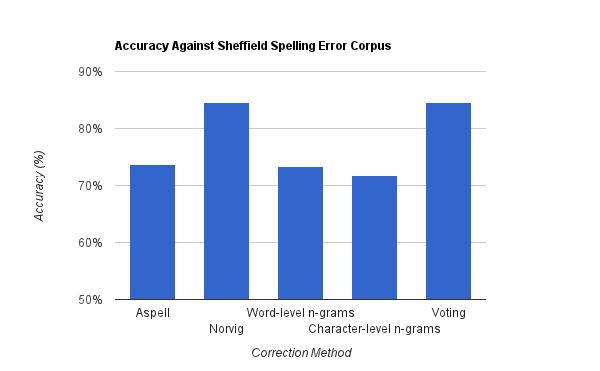
\includegraphics[scale=0.65]{images/sheffieldaccuracy}
	\caption{Graph showing the accuracy of each of the spelling correction methods against the Sheffield University spelling error corpus}
\end{figure}

\subsubsection*{Aspell Accuracy Results}
A surprising result from this investigation was the comparatively low score of 73.7\% for the Aspell software on this evaluation set. Aspell is a well regarded spelling error correction software that is used by many people, particularly in Unix environments. Aspell seemed to have difficulty with errors that contain sounds that are slightly different from the sounds in the correct correction. This problem was due to the method that Aspell uses for correction that ranks possible correction candidates based on how close they sound rather than how close they are spelled.

Another problem Aspell seemed to have was with words that were made up of two correctly spelled words concatenated together. Aspell tended to suggest splitting the words into the two constituent words instead of keeping them together. One example of this is with the spelling error \emph{``exta"} which Aspell corrected to \emph{``ex ta"} instead of, the correct, \emph{``extra"}. One explanation for this is that the edit value for splitting a word in two is less than that of a letter insertion meaning that a split will always be favoured over an insertion.

\subsubsection*{Norvig's Noisy Channel Method Accuracy Results}
Using the spelling error to correction mappings we see that Norvig's noisy channel method for spelling error correction performs best with 84.6\% accuracy. In the Sheffield corpus most of the errors are one edit distance away from a correctly spelled word and Norvig's high rate of accuracy can be attributed to the algorithm's method which makes the assumption that most spelling errors occur within only one character distance from a correctly spelled word. Some examples of words that Norvig's algorithm got incorrect were:
\begin{itemize}
\item Corrected ommissions to commissions but correct result was omissions
\item Corrected potentialy to potential but correct result was potentially
\item Corrected heuritics to heuritics but correct result was heuristics
\end{itemize}
The errors in Norvig's method can be explained by the dictionary used to store correct words and their probability of appearing in a text. As Norvig's method ranks possible corrections based on these probabilities, a lot of the accuracy of correction balances on the contents of the dictionary and whether there were more occurrences of a particular word in the training texts provided at the training stage.

\subsubsection*{Character-Level N-Gram Method Accuracy Results}
Unfortunately, the character-level n-gram method did not perform particularly well in comparison to the other methods with an accuracy of 71.7\%. Examples of some errors when using this method were:
\begin{itemize}
\item Corrected homr to homer but correct result was home
\item Corrected wiil to wil but correct result was will
\item Corrected tiem to tie but correct result was item
\end{itemize}
The above results suggest that the character-level n-gram method seems to favour shorter corrections over the longer correct correction. This can be explained by the scoring method which assigns a smaller number of n-grams to the shorter word meaning the correction has to match fewer n-grams to receive a higher score than a longer word. This is obviously a weakness of the algorithm and leads to an accuracy far below an acceptable level for any spelling error corrector. Another weakness of this system is the requirement that a correction must share many of the same n-grams as a correct word. This requirement means that errors that are caused by the switching of letters will result in different n-grams and the system will be less likely to find the correction.

\subsubsection*{Word-Level N-Gram Method Accuracy Results}
The final singular method of spelling error correction was the word-level n-gram correction method which requires context to work correctly. In the case of this experiment there was no context that could be used for each of the corrections and so a blank context was given at each step in the evaluation. By giving the algorithm no context to work with it produced roughly similar answers to the other isolated error correction methods described above and achieved an accuracy percentage of 73.4\%.

\subsubsection*{Voting Algorithm Accuracy Results}
The idea behind using a voting algorithm was that the system would have a greater accuracy than the sum of its parts. Investigating this claim using the Sheffield spelling error corpus we see that the voting algorithm performs at least as well as its best performing sub-algorithm with an accuracy rate of 84.6\%. Example output from the voting algorithm is given below:
\begin{itemize}
\item {[`facilities', `facilities', `facilities']} which gave the correct output of facilities
\item {[`worth', `worst', `worth']} which gave the correct output of worth
\item {[`similarly', `similarity', `similarly']} which gave the incorrect output of similarly
\end{itemize}
The strikingly similar accuracy rate for the voting algorithm and the Norvig noisy channel method occurred because the Norvig algorithm achieved 84.6\% on the same errors and without the necessary context the word-level n-gram method produced very similar results to the Norvig algorithm. For this reason, most of the time there will be at least two outputs from two algorithms that produce the same answer and therefore the voting algorithm had the same accuracy as the Norvig noisy channel correction method.

\subsubsection*{Execution Time}
While performing the previous investigations the execution time was also recorded for each of the methods while correcting the Sheffield spelling error corpus. For spelling correction it is essential that time of correction is as small as possible so that users can have their spelling corrected as quickly as possible and, in the case of Tweet correction, that as many Tweets can be corrected in a short a time as possible. The time for execution for each method was as follows: 

\begin{figure}[H]
	\centering
	\label{fig:timechart}
	\includegraphics[scale=0.6]{images/executiontime}
	\caption{Time of execution for each correction method on the Sheffield corpus.}
\end{figure}

The time for execution for Norvig's noisy channel method and word-level n-grams were much lower than for the other methods. This dramatic difference in execution time between the methods can be explained by the way they each interact with the dictionary. The comparatively large execution time for the character-level n-gram method was due to the need to search through every entry in the dictionary to find the closest real word for a given error. Conversely, as Norvig's noisy channel method and the word-level n-grams method generated possible corrections first and then performed a lookup on the dictionary it was a much quicker process as only a small subset of the dictionary needed to be checked.

For the voting algorithm the time for execution was simply the time it took for every method that comprises the voting algorithm to produce a suggestion and very little extra time above that to decide between the different suggestions. For this reason, the main factor in the execution time for the voting algorithm was the character-level n-grams method.

\subsection{Overall Conclusion}
Overall Norvig's noisy channel modelling method and the combined voting algorithm performed best, with respect to accuracy, on the test set of spelling error mappings. This accuracy was almost almost 10\% greater than all of the other spelling error correction methods. While the time for execution was much greater for the voting algorithm than the other methods, it still fell within an acceptable time that would not hinder the correction experience for the user. Following from the results of the experiments, it was decided that the voting algorithm would offer the best chance of producing the highest accuracy within an acceptable time when applied to Tweets and should therefore be used in the future investigations.

\section{Accuracy on Tweets}
The main goal of this project was to design and implement a system that could perform with the best possible accuracy in correcting Tweets from Twitter. For that reason, it was an obvious choice to measure the accuracy of correction on real Tweets to ensure that the system designed was of a high standard.

\subsection{Methods of Experimentation}
To explore the accuracy of the voting algorithm, which performed best on generic spelling error correction in the previous section, a comparison was made with the existing Aspell spelling error correction software on three sets of 100 Tweets. The test set of Tweets included the corrected version of the Tweet alongside the original Tweet as found in the Tweet corpus. The evaluation metric as described in section \ref{eval} was then applied to each Tweet and an overall percentage accuracy was reported for each of the methods.

The test sets used for the evaluation can be found in the appendix.

\subsection{Results}
The results of the investigation are presented in the graph below:

\begin{figure}[H]
	\centering
	\label{fig:accuracychart}
	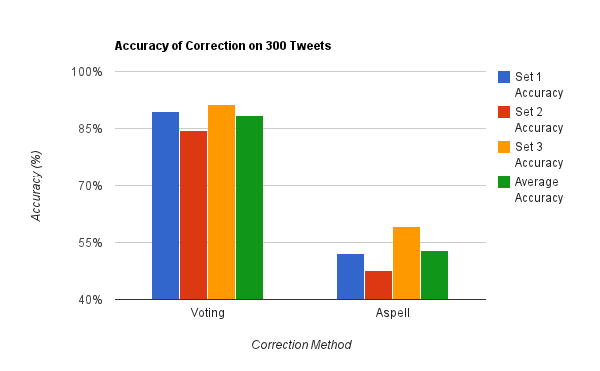
\includegraphics[scale=0.6]{images/accuracychart}
	\caption{Results of accuracy evaluation on new voting algorithm and Aspell.}
\end{figure}

The results clearly show a large 35.5\% increase in average accuracy over the 300 Tweets for the novel voting algorithm presented in this report. At its largest, the difference between the existing Aspell system and the new voting algorithm was 37.3\% which suggests a significant increase in spelling quality was obtained. The results and consequences of the experiment are further discussed in section \ref{analysisT}.

\subsection{Analysis}
\label{analysisT}
Along with the percentage similarity, the evaluation system also outputs the differences between the expected output from the error correction and the actual output from the correction system. This extra output allowed for error analysis to be performed on the output for both systems to highlight the areas of common mistakes in their correction. Additionally, the output from the error analysis could be used to increase accuracy of the voting algorithm to ensure that the voting algorithm was producing the best possible results.

An example output from the evaluation program when applied to output gained from the voting algorithm is presented below:
\begin{figure}[H]
	\centering
	\label{fig:output}
	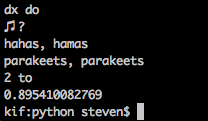
\includegraphics{images/sampleoutput}
	\caption{Sample evaluation output of voting algorithm.}
\end{figure}

For this example, the output of the voting algorithm on set 1 \ref{} was tested against the corrected version of set 1 \ref{}. In figure \ref{fig:output}, the expected output of the system is given on the left and the actual output for the system is on the right. The last value is the total accuracy of the correction as a function of the total number of words in the Tweets corrected and the number of accurate error corrections.

\subsubsection*{Tweet-specific Features and Non-English Language Errors}
The biggest difference in errors from the Aspell program that were correctly handled by the voting algorithm were the Tweet specific features such as URLs, \emph{#Hashtags}, \emph{@Usernames}, and \emph{Re-Tweets}. Obviously, without any special treatment the Aspell program handled all text it was given as letters and words and then tried to correct them. This produced results such as \emph{``href"}, the term to signify a link, being corrected to \emph{``ref"} which if left in this way would break any future uses for the link in the Tweet as there would be no way to know what a link was. While correcting Tweets, Aspell also highlighted \emph{\#Hashtags} and \emph{@Usernames} as spelling errors in the source. Luckily, in these cases as there were no words that could possibly contain \emph{@} or \emph{\#}, the Aspell system ignored the errors and left them as they appeared.

Another large difference between the results of the Aspell program and the new voting algorithm was in the correction of languages other than English. When faced with a language other than English, such as those found in a large number of the Tweet collection, Aspell attempts to correct them to their closest English word in terms of edit distance. This produced errors that would hinder the use of non-English language Tweets in further studies as the original language will not be maintained. On the other hand, as the voting algorithm contains a condition that breaks further correction if it detects a large number of corrections required it is possible to keep the original language intact. Unfortunately, around 20\% of all errors made by the voting algorithm were caused by the simplistic language detection but as the number of total errors made by the voting algorithm is relatively small, compared to Aspell, the total effect on the quality of correction was thought to be negligible.

A solution for the errors caused by the non-English language detection could come in two forms, by either: performing a more accurate method of language detection, or using a language independent spelling error correction method. For language detection the work of Cavnar and Trenkle \cite{}, which uses statistics to calculate which language a text belongs to, could be used to detect languages before any spelling error correction has taken place saving time and effort. For language independent spelling error correction many examples of languages must be provided but once training has taken place a system can be built that doesn't require any extra information \cite{GOOGLE}.

\subsubsection*{Contraction Errors}
With Tweets a common occurrence is the shortening of longer words in order to fit as much content as possible into the 140 character limit. When contractions were found in the Tweets by Aspell, it attempted to correct them using the same method as it used for all other words. Using this method it found the correct words in its dictionary that were closest to what it thought was an error. Without the extra knowledge of the fact that some of the errors might actually be a contraction this produced many errors in the correction. While the Aspell software struggled to correct contractions the voting algorithm was built with contractions in mind at the design stage. Through careful analysis of the errors in correction for the voting algorithm a selection of commonly used contractions was compiled and inserted into the algorithm so that when one of the contractions is encountered it is simply replaced with the full word. Overall, this method in the new voting algorithm worked well on contractions that are unambiguous such as \emph{``u"} to \emph{``you"} but can incorrectly change a contraction when it is ambiguous what word the user means to shorten. Ambiguous contractions include the number \emph{``2"} in which the user might have meant \emph{``to"}, \emph{``too"}, or it might not have been a contraction at all and they meant to use the number 2. The ambiguous correction problem occurred around 6\% of the time when evaluating the three evaluation sets and could therefore be described as not a significant problem.

A solution to the ambiguous contraction correction could be to perform more natural language processing techniques to ascertain which of the possible contraction correction the user meant using the context of the word, for example. This could be easily incorporated into the existing context-sensitive error correction method which is one part of the voting system presented throughout this report.

\subsubsection*{Single Edit Correction Errors}
One area that the new voting algorithm performed well in is when the error is only one character away from being a correctly spelled word. Commonly occurring word usage on Twitter such as dropping the final \emph{``g"} from words that end in \emph{``ing"} were accurately corrected around 90\% of the time. Other errors that are only one edit unit away from a correct word didn't fair quite as well as with the \emph{``ing"} words. It was a particular problem for shorter words as due to their length not enough information was available and they could be classified more easily as an incorrect word than a longer word with only one edit distance unit away which will have more correct characters and will likely be corrected accurately.

\subsubsection*{Dictionary Errors}
The dictionary of the spelling error corrector is a fundamental factor in the accuracy that the particular system can obtain. With respect to the new voting algorithm, one area of failing in the system was with it not recognising more commonly used conversational words. Conversational words are words that a person is more likely to use in personal communication with someone rather than in writing formally for an article for example. With Twitter being a form of communication between people a lot of people use many of these conversational words. The voting system and the Aspell system did not perform as well with colloquial language. Almost 40\% of the errors in correction by the new voting algorithm were caused by the system not being aware of these conversational and more modern words. Words such as \emph{``lol"}, \emph{``lmao"}, or even \emph{``tweet"} are not commonly used in writing and would therefore not be found in texts used for training a spelling error correction system. As these words were not found in either the voting system's or Aspell's dictionary both inaccurately corrected them which lowered the quality of the correction, particularly in the case of Aspell.

Errors caused by dictionaries are difficult problems to solve due to the constantly evolving languages of humans creating new words, removing old words, or incorporating new words from other languages. For this reason, a static dictionary would never be able to be used for 100\% accuracy in spelling error correction. One possible technique for achieving excellent accuracy would be to use the power and size of the Internet to create a constantly evolving dictionary that changes along with the language that people are using. This system could easily be incorporated into the existing voting algorithm, as presented in this report, as it is fully independent towards the dictionary provided and will work with whatever data is given to it.

\subsubsection*{Language Errors}
One area where Aspell performed better than the new voting algorithm was when spelling errors occurred by the concatenation of two correctly spelled words. For example, the word \emph{``myheart"} is an error but it's actually made up of two correctly spelled words \emph{``my"} and \emph{``heart"}. Aspell can successfully recognise that the error is, in fact, two words concatenated but none of the individual algorithms that make up the complete voting algorithm handle this and will attempt to correct the word as a whole. Although Aspell can recognise the error it also tends to find that an error has been concatenated when it was not, leading to many false positives where it will split an error into two words incorrectly.

Ambiguity in what a spelling error is was also a source of error in both the Aspell system and the voting system. Both systems use their respective dictionaries to highlight which words are most likely errors by finding the words that don't exist within in the dictionary. While this may work for most errors, it will not find any spelling errors that form another real word. This is a problem for both systems but it could be rectified by using more linguistic properties and methods that take into account the context of the word as well as or instead of whether a word is contained in a dictionary.

The final source of errors in the voting algorithm were when users elongated a correctly spelled word, for example, by repeating a single letter multiple times in a word. Common words found in Tweets were usually exclamations such as \emph{``yeaaaaaah"} and \emph{``nooooooo"}. In these examples, the letter \emph{``a"} and the letter \emph{``n"}, respectively, have been repeated multiple times to convey a stronger feeling. With the voting algorithm looking for words in a dictionary that were closest, in terms of edit distance, to the error the length of the word can have a great effect on the accuracy. For example, the words closest to \emph{``yeaaaaaah"} will be words of length 9$\pm$1, which is too far away for the accurate correction \emph{``yeah"} which has a length of 4.

\subsection{Overall Conclusion}
This investigation aimed to quantify the accuracy of our novel voting algorithm for spelling correction when applied to Tweets from Twitter. A manually corrected version of the Tweets was also created to be able to calculate how accurate the algorithm was. To offer a fair comparison between existing spelling error correction systems the Aspell software was used to correct the same set of Tweets and compared against the same manually corrected Tweet set. 

While there were some problems in the results of using our novel voting algorithm for correcting Tweets, the accuracy still achieved better accuracy than Aspell by 35\% on average which is a significant difference in quality. This increase in accuracy would allow future users of the data to be confident in the spelling of the Tweets.

\section{Training a System Using Tweets}
As the system was built incorporating the new voting algorithm for spelling error correction used knowledge it learned from sources of text that was given to it, the accuracy of the system could be affected by the quality, size, and content of the texts it has learned from. Following from this, an important investigation to perform was how much the accuracy of the system was affected by the choice of training texts.

From this it was decided that an important area to investigate was whether it was possible to train the system using Tweets as the training text. By using Tweets to train the system it meant that it could learn the intricacies of the language used in Twitter without human intervention and could provide corrections that were tailored to Twitter-specific text.

\subsection{Methods of Experimentation}
To train the system the selection of Tweets to use was imperative to the possible quality of the Tweet-trained voting system. As there was such a large selection of over 98 million Tweets available, it was important to not lose the variety of Tweets while ensuring the running time of both the training and evaluation did not take an excessive time. It was decided to use 5 million Tweets which, based on the average Tweet length of 14.98 \cite{}, would give around 75 million words to learn and produce a dictionary from.

The system was then trained on all the Tweets; whether they contained spelling errors or were of the English or not. When running the experiments the idea was that the noise created from spelling mistakes in the training Tweets would be removed by the volume of Tweets by applying a threshold for the word frequency which was set at 50. The number 50 was selected as a trade-off between less common words making it into the dictionary and spelling errors not making it into the dictionary.

Evaluating the accuracy of the newly Tweet-trained system was performed in the same way as in the previous experiment by using the same Tweets and the set of manually corrected Tweets. Using the same evaluation set as before ensured it was possible to fairly compare the results of the Tweet-trained system with the system trained using the newswire texts.

\subsection{Results}
The results of the investigation are presented in the graph below:
\begin{figure}[H]
	\centering
	\label{fig:tweetaccuracy}
	\includegraphics[scale=0.6]{images/tweetsaccuracy}
	\caption{Results of accuracy evaluation with new voting algorithm trained using 5 million Tweets.}
\end{figure}
With the new Tweet-trained voting algorithm, the spelling error correction system achieved accuracies of 90.1\%, 84.0\%, and 89.4\% with an average accuracy of 87.8\%. The corresponding accuracies for the original newswire-trained system were 89.5\%, 84.6\%, and 91.3\% with an average accuracy of 88.5\%. The implications of the results found in this experiment are discussed in section \ref{tweetanalysis}.

\subsection{Analysis}
\label{tweetanalysis}
The accuracy of the Tweet-trained system matched the accuracy achieved by the original system that was trained using traditional clean newswire text within 1\%. Such a small difference in accuracy compared to the newswire-trained system was an interesting result. Training a Twitter spelling error correction system to correct Tweets based on other examples of Tweets was an exciting result as this technique can be extended to build other domain specific spelling error correction systems without finding other sources of plain text, saving time and effort.
